\documentclass{standalone}
\usepackage{tikz}
\usetikzlibrary{patterns, positioning}

\begin{document}
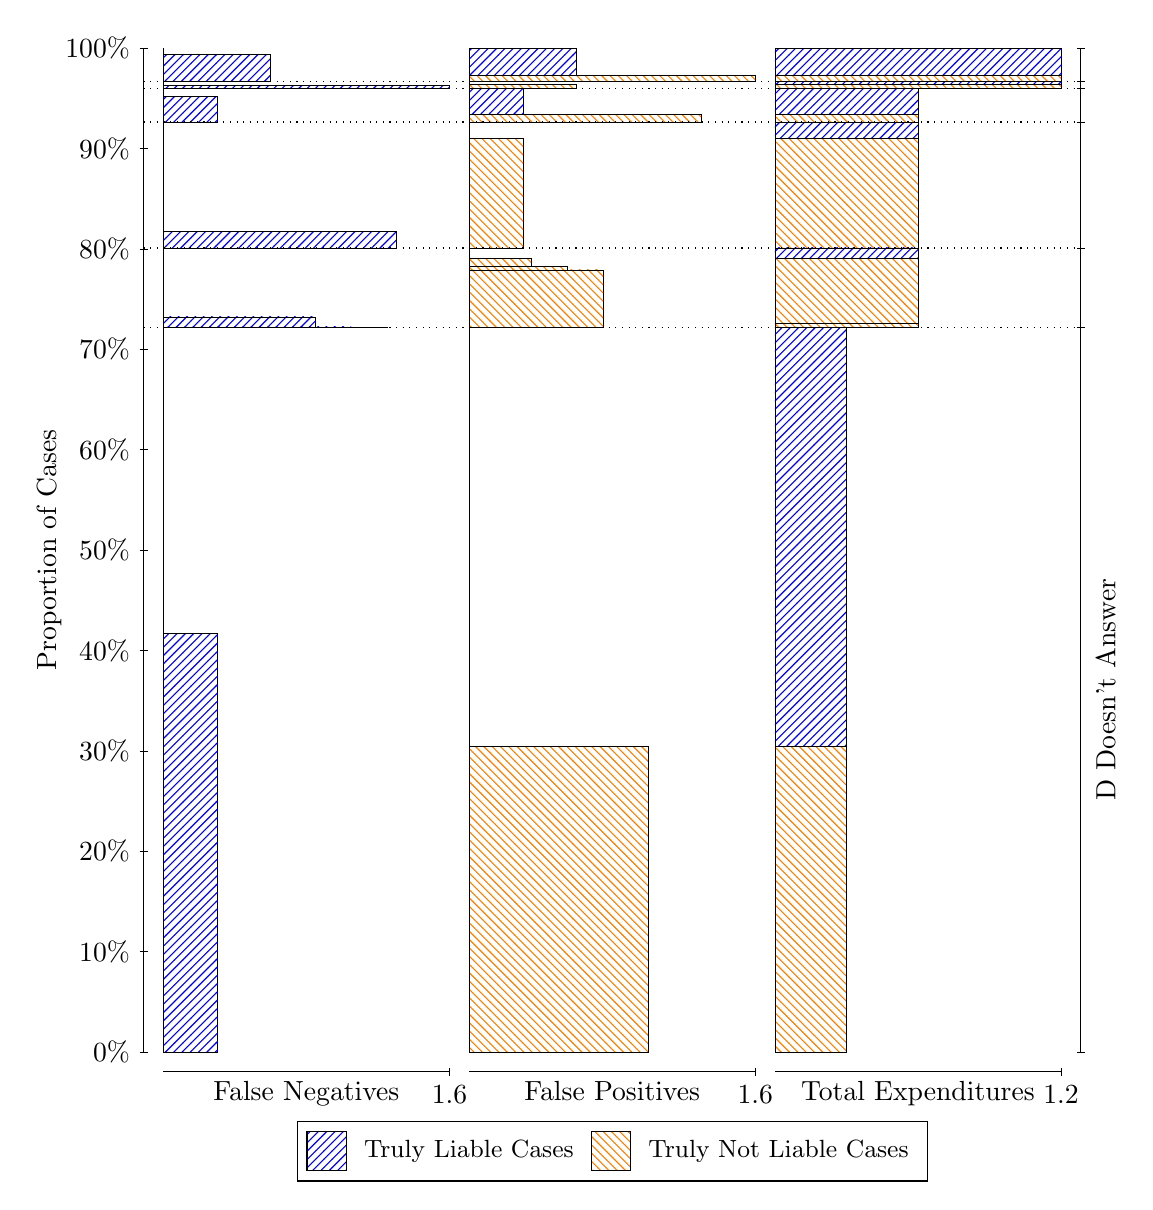
\begin{tikzpicture}
\draw[black, very thin] (1.5,1.75) -- (1.5,14.5);
\node[rotate=90, anchor=center] at (0.3, 8.125) {Proportion of Cases};
\draw[black, very thin] (1.45,1.75) -- (1.55,1.75);
\node[anchor=east] at (1.45, 1.75) {0\%};
\draw[black, very thin] (1.45,3.025) -- (1.55,3.025);
\node[anchor=east] at (1.45, 3.025) {10\%};
\draw[black, very thin] (1.45,4.3) -- (1.55,4.3);
\node[anchor=east] at (1.45, 4.3) {20\%};
\draw[black, very thin] (1.45,5.575) -- (1.55,5.575);
\node[anchor=east] at (1.45, 5.575) {30\%};
\draw[black, very thin] (1.45,6.85) -- (1.55,6.85);
\node[anchor=east] at (1.45, 6.85) {40\%};
\draw[black, very thin] (1.45,8.125) -- (1.55,8.125);
\node[anchor=east] at (1.45, 8.125) {50\%};
\draw[black, very thin] (1.45,9.4) -- (1.55,9.4);
\node[anchor=east] at (1.45, 9.4) {60\%};
\draw[black, very thin] (1.45,10.675) -- (1.55,10.675);
\node[anchor=east] at (1.45, 10.675) {70\%};
\draw[black, very thin] (1.45,11.95) -- (1.55,11.95);
\node[anchor=east] at (1.45, 11.95) {80\%};
\draw[black, very thin] (1.45,13.225) -- (1.55,13.225);
\node[anchor=east] at (1.45, 13.225) {90\%};
\draw[black, very thin] (1.45,14.5) -- (1.55,14.5);
\node[anchor=east] at (1.45, 14.5) {100\%};

\draw[black, very thin] (13.4,1.75) -- (13.4,14.5);
\draw[black, very thin] (13.35,1.75) -- (13.45,1.75);
\node[anchor=west] at (13.35, 1.75) {};
\draw[black, very thin] (13.35,10.952) -- (13.45,10.952);
\node[anchor=west] at (13.35, 10.952) {};
\draw[black, very thin] (13.35,11.961) -- (13.45,11.961);
\node[anchor=west] at (13.35, 11.961) {};
\draw[black, very thin] (13.35,13.56) -- (13.45,13.56);
\node[anchor=west] at (13.35, 13.56) {};
\draw[black, very thin] (13.35,13.983) -- (13.45,13.983);
\node[anchor=west] at (13.35, 13.983) {};
\draw[black, very thin] (13.35,14.078) -- (13.45,14.078);
\node[anchor=west] at (13.35, 14.078) {};
\draw[black, very thin] (13.35,14.5) -- (13.45,14.5);
\node[anchor=west] at (13.35, 14.5) {};

\draw[black, very thin, pattern color=blue, pattern=north east lines] (1.75,1.75) rectangle (2.4312,7.0692);
\draw[black, very thin, pattern color=orange, pattern=north west lines] (1.75,7.0692) rectangle (1.75,10.952);
\draw[black, very thin, pattern color=blue, pattern=north east lines] (1.75,10.952) rectangle (4.5885,10.956);
\draw[black, very thin, pattern color=blue, pattern=north east lines] (1.75,10.956) rectangle (4.1344,10.958);
\draw[black, very thin, pattern color=blue, pattern=north east lines] (1.75,10.958) rectangle (3.6802,11.085);
\draw[black, very thin, pattern color=orange, pattern=north west lines] (1.75,11.085) rectangle (1.75,11.961);
\draw[black, very thin, pattern color=blue, pattern=north east lines] (1.75,11.961) rectangle (4.7021,12.169);
\draw[black, very thin, pattern color=orange, pattern=north west lines] (1.75,12.169) rectangle (1.75,13.56);
\draw[black, very thin, pattern color=blue, pattern=north east lines] (1.75,13.56) rectangle (2.4312,13.888);
\draw[black, very thin, pattern color=orange, pattern=north west lines] (1.75,13.888) rectangle (1.75,13.983);
\draw[black, very thin, pattern color=blue, pattern=north east lines] (1.75,13.983) rectangle (5.3833,14.027);
\draw[black, very thin, pattern color=orange, pattern=north west lines] (1.75,14.027) rectangle (1.75,14.078);
\draw[black, very thin, pattern color=blue, pattern=north east lines] (1.75,14.078) rectangle (3.1125,14.421);
\draw[black, very thin, pattern color=orange, pattern=north west lines] (1.75,14.421) rectangle (1.75,14.5);
\draw[black, very thin, pattern color=orange, pattern=north west lines] (5.6333,1.75) rectangle (7.9042,5.6329);
\draw[black, very thin, pattern color=blue, pattern=north east lines] (5.6333,5.6329) rectangle (5.6333,10.952);
\draw[black, very thin, pattern color=orange, pattern=north west lines] (5.6333,10.952) rectangle (7.3365,11.681);
\draw[black, very thin, pattern color=orange, pattern=north west lines] (5.6333,11.681) rectangle (6.8823,11.729);
\draw[black, very thin, pattern color=orange, pattern=north west lines] (5.6333,11.729) rectangle (6.4281,11.828);
\draw[black, very thin, pattern color=blue, pattern=north east lines] (5.6333,11.828) rectangle (5.6333,11.961);
\draw[black, very thin, pattern color=orange, pattern=north west lines] (5.6333,11.961) rectangle (6.3146,13.352);
\draw[black, very thin, pattern color=blue, pattern=north east lines] (5.6333,13.352) rectangle (5.6333,13.56);
\draw[black, very thin, pattern color=orange, pattern=north west lines] (5.6333,13.56) rectangle (8.5854,13.655);
\draw[black, very thin, pattern color=blue, pattern=north east lines] (5.6333,13.655) rectangle (6.3146,13.983);
\draw[black, very thin, pattern color=orange, pattern=north west lines] (5.6333,13.983) rectangle (6.9958,14.034);
\draw[black, very thin, pattern color=blue, pattern=north east lines] (5.6333,14.034) rectangle (5.6333,14.078);
\draw[black, very thin, pattern color=orange, pattern=north west lines] (5.6333,14.078) rectangle (9.2667,14.157);
\draw[black, very thin, pattern color=blue, pattern=north east lines] (5.6333,14.157) rectangle (6.9958,14.5);
\draw[black, very thin, pattern color=orange, pattern=north west lines] (9.5167,1.75) rectangle (10.425,5.6329);
\draw[black, very thin, pattern color=blue, pattern=north east lines] (9.5167,5.6329) rectangle (10.425,10.952);
\draw[black, very thin, pattern color=orange, pattern=north west lines] (9.5167,10.952) rectangle (11.333,10.999);
\draw[black, very thin, pattern color=blue, pattern=north east lines] (9.5167,10.999) rectangle (11.333,11.001);
\draw[black, very thin, pattern color=orange, pattern=north west lines] (9.5167,11.001) rectangle (11.333,11.83);
\draw[black, very thin, pattern color=blue, pattern=north east lines] (9.5167,11.83) rectangle (11.333,11.961);
\draw[black, very thin, pattern color=orange, pattern=north west lines] (9.5167,11.961) rectangle (11.333,13.352);
\draw[black, very thin, pattern color=blue, pattern=north east lines] (9.5167,13.352) rectangle (11.333,13.56);
\draw[black, very thin, pattern color=orange, pattern=north west lines] (9.5167,13.56) rectangle (11.333,13.655);
\draw[black, very thin, pattern color=blue, pattern=north east lines] (9.5167,13.655) rectangle (11.333,13.983);
\draw[black, very thin, pattern color=orange, pattern=north west lines] (9.5167,13.983) rectangle (13.15,14.034);
\draw[black, very thin, pattern color=blue, pattern=north east lines] (9.5167,14.034) rectangle (13.15,14.078);
\draw[black, very thin, pattern color=orange, pattern=north west lines] (9.5167,14.078) rectangle (13.15,14.157);
\draw[black, very thin, pattern color=blue, pattern=north east lines] (9.5167,14.157) rectangle (13.15,14.5);
\draw[black, dotted] (1.5,10.952) -- (13.4,10.952);
\draw[black, dotted] (1.5,11.961) -- (13.4,11.961);
\draw[black, dotted] (1.5,13.56) -- (13.4,13.56);
\draw[black, dotted] (1.5,13.983) -- (13.4,13.983);
\draw[black, dotted] (1.5,14.078) -- (13.4,14.078);
\draw[black, very thin] (1.75,1.5) -- (5.3833,1.5);
\node[anchor=north] at (3.5667, 1.5) {False Negatives};
\draw[black, very thin] (5.3833,1.45) -- (5.3833,1.55);
\node[anchor=north] at (5.3833, 1.45) {1.6};

\draw[black, very thin] (5.6333,1.5) -- (9.2667,1.5);
\node[anchor=north] at (7.45, 1.5) {False Positives};
\draw[black, very thin] (9.2667,1.45) -- (9.2667,1.55);
\node[anchor=north] at (9.2667, 1.45) {1.6};

\draw[black, very thin] (9.5167,1.5) -- (13.15,1.5);
\node[anchor=north] at (11.333, 1.5) {Total Expenditures};
\draw[black, very thin] (13.15,1.45) -- (13.15,1.55);
\node[anchor=north] at (13.15, 1.45) {1.2};

\node[black, centered, rotate=90] at (13.72, 6.3511) {D Doesn't Answer};






\draw (7.449999999999999,1.5) node[draw=none] (baseCoordinate) {};
\begin{scope}[align=center]
        \matrix[scale=0.5, draw=black, below=0.5cm of baseCoordinate, nodes={draw}, column sep=0.1cm]{
            \node[rectangle, draw, minimum width=0.5cm, minimum height=0.5cm, pattern=north east lines, pattern color=blue] {}; &
            \node[draw=none, font=\small] (B) {Truly Liable Cases}; &
            \node[rectangle, draw, minimum width=0.5cm, minimum height=0.5cm, pattern=north west lines, pattern color=orange] {}; &
            \node[draw=none, font=\small] (B) {Truly Not Liable Cases}; \\
            };
\end{scope}

\end{tikzpicture}
\end{document}